%%=============================================================================
%% Methodologie
%%=============================================================================

\chapter{\IfLanguageName{dutch}{Methodologie}{Methodology}}%
\label{ch:methodologie}

%% In dit hoofstuk geef je een korte toelichting over hoe je te werk bent
%% gegaan. Verdeel je onderzoek in grote fasen, en licht in elke fase toe wat
%% de doelstelling was, welke deliverables daar uit gekomen zijn, en welke
%% onderzoeksmethoden je daarbij toegepast hebt. Verantwoord waarom je
%% op deze manier te werk gegaan bent.
%% 
%% Voorbeelden van zulke fasen zijn: literatuurstudie, opstellen van een
%% requirements-analyse, opstellen long-list (bij vergelijkende studie),
%% selectie van geschikte tools (bij vergelijkende studie, "short-list"),
%% opzetten testopstelling/PoC, uitvoeren testen en verzamelen
%% van resultaten, analyse van resultaten, ...
%%
%% !!!!! LET OP !!!!!
%%
%% Het is uitdrukkelijk NIET de bedoeling dat je het grootste deel van de corpus
%% van je bachelorproef in dit hoofstuk verwerkt! Dit hoofdstuk is eerder een
%% kort overzicht van je plan van aanpak.
%%
%% Maak voor elke fase (behalve het literatuuronderzoek) een NIEUW HOOFDSTUK aan
%% en geef het een gepaste titel.

% \lipsum[21-25]

\section{Fasering van de bachelorproef}%
\label{sec:fasering_bap}

Deze bachelorproef werd uitgevoerd in de volgende fases, van 9 februari (week 1) t.e.m. 22 mei (week 15), 2026:

\begin{itemize}
  \item{\nameref{sec:fase_literatuurstudie}}
  \item{\nameref{sec:fase_evaluatie_beschikbare_tools}}
  \item{\nameref{sec:fase_ontwerp_manuele_testomgeving}}
  \item{\nameref{sec:fase_implementatie_manuele_testomgeving}}
  \item{\nameref{sec:fase_opstellen_testcases}}
  \item{\nameref{sec:fase_ontwikkeling_poc}}
  \item{\nameref{sec:fase_uitvoeren_testcases}}
\end{itemize}

Indien een fase begint met hetzelfde nummer maar eindigt met een andere letter, indiceert dit dat ze op hetzelfde moment beginnen en parallel worden uitgevoerd.

Aangezien sommige fases afhankelijk zijn van elkaar en/of korter op elkaar vallen, zullen deze voor dit document in de volgende overkoepelende hoofdstukken omvat worden:

\begin{itemize}
  \item{Hoofdstuk~\ref{ch:manuele_testomgeving}: \nameref{ch:manuele_testomgeving}}
  \item{Hoofdstuk~\ref{ch:poc}: \nameref{ch:poc}}
  \item{Hoofdstuk~\ref{ch:testcases}: \nameref{ch:testcases}}
\end{itemize}

\begin{figure}[H]
  \centering
  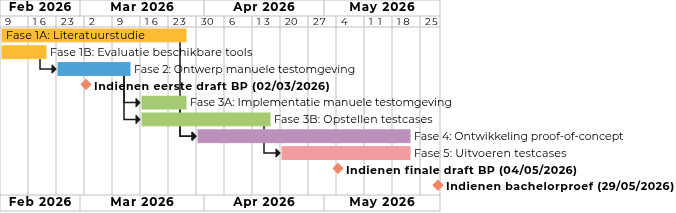
\includegraphics[width=\textwidth]{../graphics/gantt-fases.png}
  \caption[\emph{GANTT}-schema (fases van de bachelorproef)]{\label{fig:gantt-fases.png}\emph{GANTT}-schema voor de verschillende fases van de bachelorproef.}
\end{figure}

\section{Fase 1A (week 1-7): Literatuurstudie}
\label{sec:fase_literatuurstudie}

Bij het begin van het onderzoek is er parallel met de andere voorbereidende fases (1-3) een studie uitgevoerd over de stand van zaken van elk vakgebied; er werd onderzocht wat de meest courante tools zijn voor \emph{UML}-modeling, \emph{Infrastructure-as-Code} en \emph{configuration management}, alsook welke vormen de \emph{Proof of Concept} kon aannemen (zijnde als \emph{transpiler} of \emph{converter}).

\section{Fase 1B (week 1-2): Evaluatie van de beschikbare tools}%
\label{sec:fase_evaluatie_beschikbare_tools}

Hier werd er een afweging gemaakt voor de beschikbare tools  in de betrokken vakgebieden (\emph{UML}-modeling, \emph{Infrastructure-as-Code} en \emph{configuration management}) die gebruikt werden tijdens de ontwikkeling van de \emph{Proof of Concept}.
De te evalueren tools voor \emph{UML}-modeling zijn \emph{PlantUML} \& \emph{MermaidJS}, voor \emph{Infrastructure-as-Code} waren dit \emph{Terraform}, \emph{OpenTofu} \& \emph{Vagrant} en voor het ``\emph{configuration management}''-gedeelte werd er gekeken naar \emph{Ansible}, \emph{Puppet} en \emph{Chef}.

\section{Fase 2 (week 3-5): Ontwerp van de manuele testomgeving}%
\label{sec:fase_ontwerp_manuele_testomgeving}

In deze fase werd de manuele testomgeving voor de \emph{Proof of Concept} ontworpen aan de hand van netwerk- en implementatiediagrammen (ontworpen met \emph{PlantUML}/\emph{MermaidJS}). In deze diagrammen worden de hardware- (aantal \emph{CPU} cores, hoeveelheid \emph{RAM}) en softwarespecificaties (\emph{packages}, \emph{services}) van elke server beschreven, alsook hoe deze met elkaar interageren.
Deze diagrammen dienen een tweevoudig doel; ze kunnen binnen de originele context van hun taal als visuele \emph{UML}-diagrammen worden gegenereerd, en ze vormen de bron-bestanden voor de \emph{Proof of Concept}, die deze zal omzetten tot ``\emph{configuration management}''-code.

\section{Fase 3A (week 6-7): Implementatie van de manuele testomgeving}%
\label{sec:fase_implementatie_manuele_testomgeving}

Tijdens deze fase werd de infrastructuur (ontworpen in fase 2) opgezet met een \emph{Infrastructure-as-Code}-tool en geconfigureerd met een ``\emph{configuration management}''-tool (\emph{Ansible}/\emph{Puppet}/\emph{Chef}). Er werd intussen ook gedocumenteerd hoe het ``\emph{configuration management}''-gedeelte werd opgezet, want dit vormt de target output voor de \emph{Proof of Concept}.

\section{Fase 3B (week 6-10): Opstellen van de testcases}%
\label{sec:fase_opstellen_testcases}

Hier werden de testcases opgesteld waaraan de \emph{Proof of Concept} moest voldoen. Deze waren gebaseerd op bestaande omgevingen binnen de opleiding \emph{Toegepaste Informatica} en buigden zich hoofdzakelijk over de mogelijke uitvoer (de \emph{playbook}, variabelen, bestanden, \ldots) en hoe goed deze werkt tegenover de originele opstellingen.

Deze fase is in de praktijk gedeeltelijk parallel verlopen met fase 4, aangezien er tijdens het ontwikkelen van de oplossing mogelijk nieuwe testcases konden ontstaan.

\section{Fase 4 (week 8-15): Ontwikkeling van de \emph{Proof of Concept}}%
\label{sec:fase_ontwikkeling_poc}

Tijdens deze fase werd de \emph{Proof of Concept} ontwikkeld, in de vorm van een \emph{transpiler} of \emph{converter}. Deze neemt als invoer de ontworpen netwerk- en implementatiediagrammen en zet ze om tot ``\emph{Infrastructure-as-Code}''- en ``\emph{configuration management}''-code als uitvoer.

Deze fase liep tot 22 mei, 2026.

\section{Fase 5 (week 11-15): Uitvoeren van de testcases}%
\label{sec:fase_uitvoeren_testcases}

Ten slotte werden de opgestelde testen uit fase 3B uitgevoerd op de (gedeeltelijk) uitgewerkte \emph{Proof of Concept}. Op basis van de resultaten zijn er beoordelingen opgesteld die aangeeft in welke mate deze oplossing erin slaagt om een werkend eindresultaat te produceren.

Nogmaals, deze fase is parallel verlopen met fase 4.
